\documentclass [11pt]{article}
\usepackage{graphicx}
\usepackage{amssymb,amsmath}
\bibliographystyle{plain}
\usepackage{url}
\usepackage[a4paper,bindingoffset=0.2in,left=0.5in,right=0.5in,top=1in,bottom=1in,footskip=.25in]{geometry}
\begin {document}

\title{Physics Behind the Simulation: A CS 296 Report by Group 24.}
\author{
    HAREN SAGA\\
    CSE\\
    120050072\\
    120050072@iitb.ac.in
      \and
    NISHANT KUMAR SINGH\\
    CSE\\    
    120050043\\
    120050043@iitb.ac.in
    \and
    VARUN TELUGUNTLA\\
    CSE\\
    120050077\\
   120050077@iitb.ac.in
}
\date{25 Jan 2014}

\maketitle

\section{Introduction}
The purpose of the report is to explain the physics behind the simulation of the three new
added objects.
\section{Physics behind the simulation.} 
\subsection{The Top Motor}
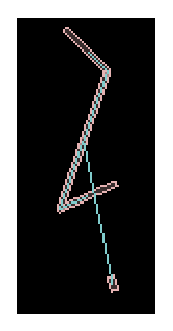
\includegraphics [scale=0.7]{xn}\\\

The bottom most part is pivoted and attached to a motor . The torque ($\tau$) supplied by the motor 
supports the motion of the system with moment of inertia ($I$). The whole system moves with an angular velocity ~\cite{hal11}.~\cite{hc11}.
\[ \tau = I* \omega \] ~\cite{tor11}.~\cite{mi11}.
The motor provides the energy for the system to be in motion.

\subsection{The Wedge($W_1$ ) on the see-saw }
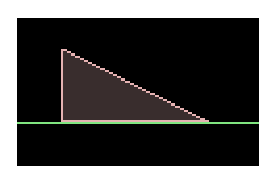
\includegraphics [scale=0.7]{w1}\\\

As the sphere ($mass - m_1$) falls on the wedge $W_1$ a horizontal impulse sets it into motion.~\cite{im11}.~\cite{coll11}.
As the wedge $W_2$ rests on the ground and the wedge $W_1$ approaches and slides off the top
in a projectile motion with a initial velocity ($v_o$) and angle ($\theta$).~\cite{hal11}.~\cite{hc11}.

Horizontal velocity remains constant.
\[v_x =  v_o Cos (\theta ) \]
Vertical velocity changes \[v_y = v_0 Sin(\theta) - g*t \]
Where $g= $acceleration due to gravity and $t$ is time.\\ ~\cite{pro11}.

\subsection{The Left Wedge($W_2$-mass $m_2$)}
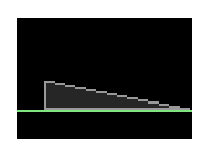
\includegraphics [scale=0.7]{w2}\\\

The wedge $W_2$ at rest ($u_2 = 0$) and the sphere (mass $m_1$ )moving with velocity ($u_1$) the final velocity of 
$W_2$ is 
\[v_2 = (\frac{2*m_1}{m_1+m_2 })*u_1\]
and that of sphere is 
\[v_1 = (\frac{2*m_2}{m_1+m_2 })*u_1\] 
and hence as $m_1 > m_2$ $W_2$ moves away faster. ~\cite{hal11}.~\cite{hc11}.~\cite{coll11}.

\section {Conclusion}
I have talked about the motion of the newly added three objects and the physics behind this motion.

\bibliography{citation}
\end{document}

